\subsection{Typical Behavior}
As discussed in the previous section, the optimum path will either take a straight line or a bracket shape. One might assume that as the variance $\sigma$ increases or the path constant $P$ decreases, the value of $\yhat$ also increases (i.e. taking wider paths around the obstacle). This is true for the most part. However, as you change the paths to try to get paths closer to the obstacle, there is a massive drop in $\yhat$ to $0$. Consider the path in Figure \ref{fig:gaussian}. With low values of $P$, $\yhat$ can be infinitely large. When $P=55$ you get a $\yhat$ of 16 (with a certain set of parameters). However, when $P=55$, the path goes straight through the obstacle ($\yhat=0$). Using Gaussian distributions, with their nicely differentiable functions, one would expect the resulting path space to be roughly continuous. However, it is not. 

\begin{figure}
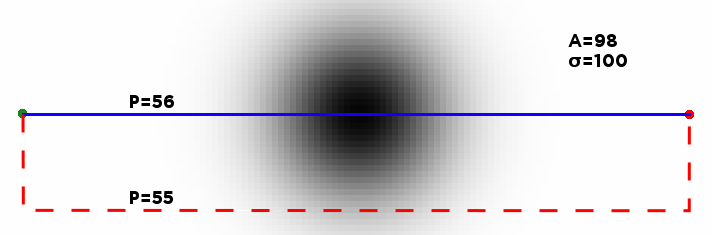
\includegraphics[width=\columnwidth]{graphix/Gaussian.png}
\caption{Gaussian Cost Function - Straight path is optimal when $P=56$, the bracket path when $P=55$. }
\label{fig:gaussian}
\end{figure}

In fact, there is no value of $P$ (with all of the other parameters remaining the same) that would result in $0<\yhat<16$. The intuition is that there is a certain value where the path planner prioritizes path length over path cost, but it is unclear why and where this happens. 





\subsection{Mathematical Explanation}
Our goal is to show why there are certain parameters that result in one of the three behaviors discussed. 
\begin{enumerate}
\item Minimum path cost is at $\yhat=0$
\item Minimum path cost is at finite $\yhat>0$
\item Minimum path cost is infinitely far away. 
\end{enumerate}

The strategy will be to estimate the relative cost of the path and then show where the local extrema are with calculus. We are forced to estimate such a cost because there is no easy way to analytically solve for a closed form of the sum over an arbitrary interval of a Gaussian. 

First, let's express the cost for the optimal path for a given the bracket shape. 
\begin{align*}
C(p_{\yhat}) =&C(segment_1) + C(segment_2) + C(segment_3) \\
C(p_{\yhat}) =&\Big[\yhat P + \sum\limits_{i=0}^{\yhat-1} f(-n, i) \Big] +
         \Big[2nP + \sum\limits_{x=-n}^{n}    f(x,\yhat) \Big]\\
     &+\Big[\yhat P + \sum\limits_{i=0}^{\yhat-1} f(n, i) \Big] \\
C(p_{\yhat}) =&(2n+2\yhat)P \\ &+\sum\limits_{i=0}^{\yhat-1} \Big[ f(-n, i) + f(n, i) \Big] + \sum\limits_{x=-n}^{n} \Big[f(x,\yhat) \Big]
\end{align*}

Now let us assume that $n$ is large enough such that the cost of segments 1 and 3 are negligible compared to $P$. We can then simplify the equation to:
\[
C(p_{\yhat}) \approx (2n+2\yhat)P +  \sum\limits_{x=-n}^{n} f(x,\yhat)
\]

Since we only care about the cost of each path in relation to other paths, let us calculate the relative cost ($RC$) of moving along the shortest path (with $\yhat=0$) and some other path where $\yhat>=0$. 
\begin{align*}
RC(\yhat) =& C(\yhat)-C(0) \\
\approx& \Big[(2n+2\yhat)P +  \sum\limits_{x=-n}^{n} f(x,\yhat) \Big] \\
 & - \Big[(2n+2(0))P +  \sum\limits_{x=-n}^{n} f(x,0) \Big] \\
\approx& 2P\yhat + \sum\limits_{x=-n}^{n} \Big[ f(x,\yhat)-f(x,0) \Big]
\end{align*}
If this quantity is negative, that means the minimum value does not occur at $\yhat=0$. Otherwise, the minimum cost path is the straight path where $\yhat=0$.

Let us now plug in the actual equation for $f$. 
\begin{align*}
RC(\yhat) \approx 2P\yhat + \sum\limits_{x=-n}^{n} \Big[ &A\exp\left(-\frac{x^2}{2\sigma^2}\right)\exp\left(-\frac{\yhat^2}{2\sigma^2}\right) -\\
                                                           &A\exp\left(-\frac{x^2}{2\sigma^2}\right) \Big] 
\end{align*}

We are faced with the sum over an interval of a Gaussian. Since $n$ is large, we can say that the costs are negligible for the cells where $x>n$, so we use the following approximation. 
\begin{align*}
        \sum\limits_{x=-n}^{n} A&\exp\left(-\frac{x^2}{2\sigma^2}\right)\exp\left(-\frac{y^2}{2\sigma^2}\right) \\
&\approx \sum\limits_{x=-\infty}^{\infty} A\exp\left(-\frac{x^2}{2\sigma^2}\right)\exp\left(-\frac{y^2}{2\sigma^2}\right)  \\
&= A\exp\left(-\frac{y^2}{2\sigma^2}\right)\sigma\sqrt{2\pi} \\
&= A\sigma\sqrt{2\pi}\exp\left(-\frac{y^2}{2\sigma^2}\right)
\end{align*}

Thus we can now approximate our relative cost. 
\[
RC(\yhat) \approx 2P\yhat + A\sigma\sqrt{2\pi} \exp\Big(\frac{-\yhat^2}{2\sigma^2}\Big) - \exp(0) ) \\
\]

We'd like to find the local extrema. To do this, we take the derivative and set it to 0. 
\begin{align}
RC'(\yhat) \approx& 2P + A\sigma\sqrt{2\pi}             \exp\Big( \frac{-\yhat^2}{2\sigma^2} \Big) \frac{-\yhat}{\sigma^2}\notag\\
0  \approx& 2P - A\sqrt{2\pi}        \frac{\yhat}{\sigma} \exp\Big( \frac{-\yhat^2}{2\sigma^2} \Big) \notag\\
  \frac{P}{A} \approx& \sqrt{\frac{\pi}{2}} \frac{\yhat}{\sigma} \exp\bigg( \frac{-1}{2} \Big(\frac{\yhat}{\sigma} \Big)^2 \bigg) 
\end{align}
\begin{figure}
\centering
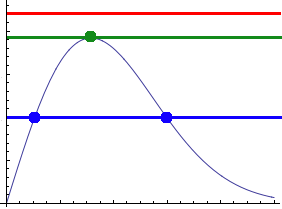
\includegraphics[width=0.4\columnwidth]{graphix/lambert.png}
\caption{Plot of $x \exp(-x^2)$, with lines marking values where the equation has no solutions (top line), one solution (middle line) or two solutions (bottom line).}
\label{fig:lambert}
\end{figure}

This equation is related to the Lambert W-function, which is rather unwieldy, and therefore has an unknown number of solutions. As seen in Figure \ref{fig:lambert}, there could be 0, 1 or 2 solutions, depending on the value of $\frac{P}{A}$. This means that the Relative Cost has critical points at those solutions and the limits. From this, there are several key observations we can make. 
\begin{enumerate}
\item Two critical points are necessary for there to be a finite $\yhat>0$, as seen in Figure \ref{fig:twosolutions}. 
\item It is not sufficient to have two critical points to cause a finite $\yhat>0$, since the minimum may not have a negative value, meaning that the optimal path will be at $\yhat=0$. Similar scenario occurs when there is only one critical point as in Figure \ref{fig:inflection}. 
\item If there are no critical points as in Figures \ref{fig:zero} and \ref{fig:infinity}, then the extrema must be at the limits. If $P>0$, you end up with a positive slope like in Figure \ref{fig:zero} and the optimal minimum cost path is at $\yhat=0$. If $P=0$, then you get a negative slope and the minimum value is at $\yhat=\infty$. This follows the intuition where if $P$ is very high, then the straight path is optimal, and if $P=0$, the path length does not matter and the path can be arbitrarily far away. 
\end{enumerate}

\begin{figure}[t]
\centering
\subfloat[Two Critical Points: $\yhat>0$]{
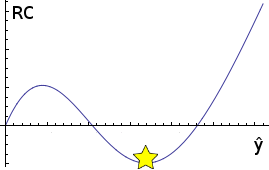
\includegraphics[width=0.4\columnwidth]{graphix/twosolutions.png}
\label{fig:twosolutions}}
\qquad
\subfloat[One Critical Point: $\yhat=0$]{
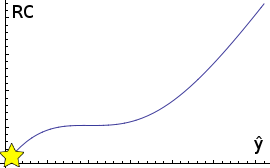
\includegraphics[width=0.4\columnwidth]{graphix/inflection.png}
\label{fig:inflection}}\\
\subfloat[No Critical Points: $\yhat=0$]{
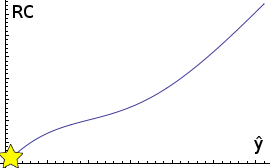
\includegraphics[width=0.4\columnwidth]{graphix/zero.png}
\label{fig:zero}}
\qquad
\subfloat[No Critical Points, $P=0$: $\yhat=\infty$]{
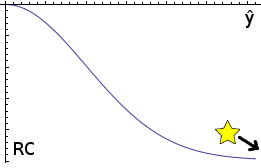
\includegraphics[width=0.4\columnwidth]{graphix/infinity.png}
\label{fig:infinity}}
\caption{Gaussian Relative Costs (y-axis) over different passing distances. Minimum cost/optimal path marked with a star. In (a), the optimum passing distance is at a finite $\yhat>0$. In (b) and (c) the optimum is at $\yhat=0$. In (d), the optimum is as far away as possible. }
\label{fig:globfig}
\end{figure}

